\documentclass[a4paper,11pt]{jlreq}
% 基本とドライバ関連
\usepackage{graphicx}
\usepackage{xcolor}
\usepackage{makeidx}
\usepackage{ascmac}

% LuaTeX-ja設定
\usepackage{luatexja}% 日本語したい
\usepackage[haranoaji,no-math,deluxe,expert,nfssonly,match,scale=1.0]{luatexja-preset}
\renewcommand{\kanjifamilydefault}{\gtdefault}% 既定をゴシック体に
\usepackage{lltjext}

% 数式系基本
\usepackage{amsmath}
\usepackage{amsthm}
\usepackage{amssymb}
\usepackage{mathtools}
\mathtoolsset{showonlyrefs=true}
\usepackage{derivative}
\usepackage[b]{esvect}
\usepackage{nicematrix}
\usepackage{siunitx}

% 画像関係
% \usepackage{animate}
\usepackage{svg}
\usepackage{tikz}

%表関連
\usepackage{multirow}

% 自然科学用追加
% \usepackage{chemmacros}
% \usechemmodule{all}
% \selectchemgreekmapping{fontspec}
\usepackage{chemfig}
% \ifdraft{}{\setchemfig{bond join=true}}
% 数式フォント設定
\newcommand{\sfscale}{0.98}
\newcommand{\ttscale}{0.96}
% \usepackage[mathnoalias]{iwona}
% \setmainfont{Iwona}
% \usepackage[scale=\sfscale]{roboto}
% \usepackage[scale=\ttscale]{roboto-mono}
% \usepackage{BOONDOX-uprscr}
% \usepackage{BOONDOX-ds}

% ページ設定
\usepackage{geometry}
\geometry{left=25truemm, right=25truemm, top=25truemm, bottom=25truemm}
% \pagestyle{empty}

% hyperref関連
\usepackage{bookmark}
\usepackage{xurl}
\hypersetup{unicode,bookmarksnumbered=true,hidelinks,final}

%%%%%%%%%%%%%%%%%%%%%%%
\graphicspath{{../figure/}}

% \setchemfig{atom sep=1.5em}

\begin{document}
高分子鎖は、模式的には「非常に細くてとても長い紐が、くるくると丸まったもの」と表現され、「このような高分子鎖の形状に起因して低分子とは大きく異なった高分子に特有な振る舞いを示す」とされている。
高分子を使いこなして特徴ある機能を発現できる材料とするためには、高分子に特有の形状をきちんと理解することが必須となるわけです。

このような高分子のイメージについて、まず、ミクロな化学構造の結合状態をみることから始めて、少しずつ理解してみよう。

\subsection{細くて長い}

高分子の例として、メチレンを繰り返し単位とした連鎖からなる最も単純な構造であるポリエチレンを対象として考えてみよう。

そのポリマーの構造は、エチレンモノマー単位が重合により多数連結した鎖であり、それぞれのモノマー単位は\chemfig{C-C}結合でつながっている。
なお、\chemfig{C-C}結合の結合長は\qty{0.154}{nm}で、3つの炭素が形成する\chemfig{C-C-C}結合は約\ang{109.5}の結合角を有している
\footnote
{
炭素原子が正四面体の重心に来るようにおいた場合に、その四つの結合のそれぞれが正四面体の頂点となるような構造を取っていることから、この結合角は理解できる。
なお、炭素の立体構造は以下となる。
\begin{center}
	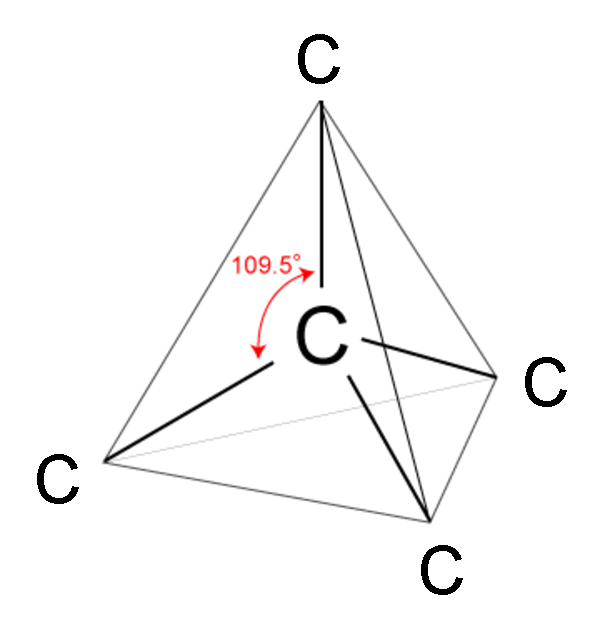
\includegraphics[width=2.5cm]{carbon.eps}
\end{center}

この結合角の具体的な導出については、 \ref{sec: carbon_BA} に示した。
}。

ここで、ポリマーの主鎖のモデルとして、まず、炭素が四個のアルキルであるブタンを考えてみよう。
真ん中の炭素結合(2位の炭素と 3位の炭素との間の結合:\chemfig{CH3-CH2-CH2-CH3})に対して、ニューマン投影式を考えると、エネルギーの低い状態として、それぞれのメチル基がトランスの位置
\footnote
{
トランス配座は、最初の三つの炭素の張る平面上で1位の炭素と4位の炭素が反対の位置(トランス)となる状態であり、ポテンシャル・エネルギーが最低となる。
}
と、ゴーシュの位置
\footnote
{
ゴーシュ配座は、トランスの位置からみて、回転角 $\phi = \pm 60^o$ に 4 位の炭素が位置する、局所的にエネルギー極小となる状態である。
この場合、1,4 位の炭素の相互作用が存在するため、トランス状態よりはエネルギーは高い。
}
になる状態を想定できることになる。
この時のエネルギー状態図も併せて、以下に示した。
\begin{figure}[htb]
 \centering
	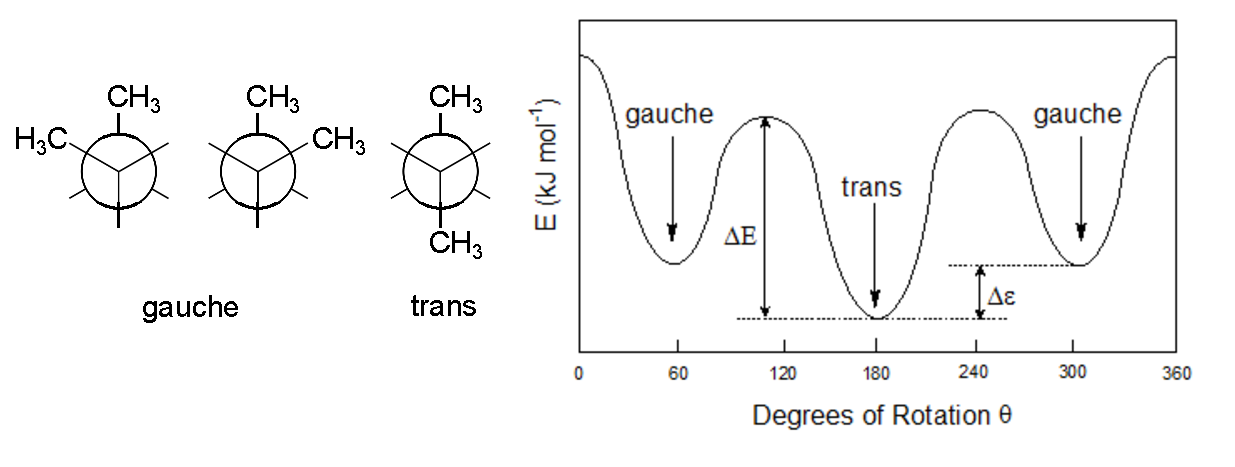
\includegraphics[width=10cm]{butane.eps}
	\caption{ブタンの配座とエネルギー状態図}
	\label{fig: butane}
\end{figure}

ブタンのモデルをベースに考えると、ポリマー主鎖は、ブタンの両端のメチル基の位置からさらに結合が伸びているものとモデル化して考えることができる。
ここで、熱的に安定な状態(よりエネルギーの低いトランス状態)の極限として主鎖の炭素が全部トランスの配置にある状態を考えると、ポリマー鎖は一つの平面上にジグザグに伸びた形(平面ジグザグ構造)となる。

簡便のために、水素を無視して、C-C 結合(結合長は 1.54 \AA)のみを考えてみよう。
このとき、ポリエチレンの直径は約 0.09 nm、また、ポリマー鎖中のモノマー単位の長さは約 0.25 nm と見積もることができる(章末問題 \ref{it:2-1})。
そして、このようなモノマー単位が、仮に、平面ジグザグ構造の連鎖として直線的につながったと考えると、例えば、ポリエチレンの分子量が 10 万であった場合には、その長さは約 900 nm となる
\footnote
{
この時、縦横比を表すアスペクトレシオを考えると、10000 ということになる。
}(章末問題 \ref{it:2-2})。

もっと手に取って扱えるような大きさで考えてみよう。
このヒモを直径 5 mm のチョークを使って横一本の線で黒板に書いたとすると、その長さは約 50 m (普通の黒板の 10 枚分程度)ということになる。
いかに高分子が細長い形状をしているかが想像できるであろう。
 


\subsection{くるくる丸まる}

高分子をピンと引き延ばすと、非常にアスペクト比の高い細長いものとなることを、上に示した。
しかしながら、自然な状態での実際の高分子は、決してこのような伸び切り構造を取っているわけではない。
ぐるぐるに丸まった、ランダムコイルと呼ばれる状態になっていることが知られている。
このことを、統計力学的な考え方で確かめてみよう。

統計力学によれば、エネルギーの異なる二つの状態(エネルギー差 $\Delta E$)の出現確率の比 $r(\Delta E)$ は、ボルツマン因子を用いて、下式のように表すことができる
\footnote
{
ボルツマン因子とは、温度 $T$ の熱平衡状態にある系において、エネルギー $E_i$ である状態 $i$ が出現する相対確率 $P(E_i)$ を、下式のように定める重み因子である。
ボルツマン因子は、通常カノニカル分布によって記述される系を議論する際に用いられる。
\begin{align*}
P(E_i) = \dfrac{1}{Z} \exp(-\beta E_i)
\end{align*}
ここで、$Z=\sum_i \exp(-\beta E_i)$ は、$\sum_i P_i = 1$ とするための規格化因子であり、分配関数、あるいは、状態和と呼ばれる。

}(章末問題 \ref{it:2-3})。
\begin{equation}
r(\Delta E) = \exp(-\beta \Delta E)=\exp \left( -\dfrac{\Delta E}{k_B T} \right)
\label{eq:ratio}
\end{equation}

ただし、$\beta=\dfrac{1}{k_B T}$、$k_B$ はボルツマン定数($k_B =1.380 \times 10^{-23} {\rm J K}^{-1}$)、$T$ は絶対温度である。

このことを利用すれば、前述のトランスとゴーシュ状態とのポテンシャル・エネルギー差 $\Delta \varepsilon$ に基づいて、熱平衡状態でのそれぞれの状態の出現確率の比を求めることができる。
トランス状態が連続する限り、ポリマー鎖は平面ジグザグ構造により直線的に伸びていくが、ゴーシュが出現することで鎖の曲りが生じる。
一般に、このエネルギー差 $\Delta \varepsilon$ は数 kJ mol$^{-1}$ 程度であるので、数個程度のモノマー単位の連鎖ごとに、ゴーシュ状態が出現、すなわち、ポリマー主鎖が曲ることになる(章末問題 \ref{it:2-4}、\ref{it:2-5})。

前述のように、ポリマー鎖は非常に細長いものであるから、10個以下の連鎖で少し曲がるような程度の曲りであっても、全体でみれば、くるくると丸まったものとなっていることが理解できる。

\subsection{ぐにゅぐにゅと蠢く}

さらに、トランス状態からゴーシュ状態へと遷移する際のエネルギー障壁($\Delta E$)を用いた考察から、この遷移の起こる頻度を見積もることも可能である。
分光学的な測定から、ブタンにおける C-C 結合周りの回転振動数は、$10^{12}$ sec$^{-1}$ のオーダーで生じることが知られている。
トランス $\leftrightarrow$ ゴーシュの相互遷移のエネルギー障壁は $10 \sim 20$ kJ mol$^{-1}$ 程度であるので、ボルツマン因子を用いて評価すると、室温での遷移は $10^{9}$ sec$^{-1}$ 程度のオーダーで生じるものと見積もることができる(章末問題 \ref{it:2-6})。

実際の高分子においては、主鎖周りの影響を受けるため、この回転運動の振動数は低いものとなり、また、エネルギー障壁も大きくなると考えられる。
しかしながら、それでも十分に高い頻度でこのような回転異性化によるコンフォメーションの変化が生じるであろうということが想像できる。
このような変化が、高分子のミクロブラウン運動と呼ばれる運動モードの起源の主要なひとつである。


	\begin{enumerate}
		\item
		\label{it:2-1}
		(モノマー単位の大きさの見積もり)\\
		文中に示したポリエチレンの平面ジグザグ構造に基づく伸び切り構造の大きさの見積もりを、具体的に説明してください。\\
		(ヒント)\\
		C-C 結合の結合長が 1.54 \AA、三つの炭素が形成する C-C-C 結合が約 $109.5^o$ の結合角ということを考慮して、平面ジグザグ構造でのモノマー二つ分の絵を書いてみれば、
		ポリマー鎖の伸長方向とそれに垂直な方向との長さが見積れます。

		\item
		\label{it:2-2}
		(伸び切り鎖の長さの見積もり)\\
		ポリエチレンの分子量が 10 万であった場合に、その平面ジグザグ構造の伸び切り鎖の長さが約 900 nm となることを、具体的に説明してください。\\
		(ヒント)\\
		分子量が 10 万であった場合に、その重合度がいくつであるかを算出すればいいだけです。

		\item
		\label{it:2-3}
		(出現確率の比)\\
		エネルギーの異なる二つの状態(エネルギー差 $\Delta E$)の出現確率の比 $r(\Delta E)$ が以下の式となることを説明してください。
		\begin{equation*}
		r(\Delta E) = \exp(-\beta \Delta E)=\exp \left( -\dfrac{\Delta E}{k_B T} \right)
		\end{equation*}
		(ヒント)\\
		熱平衡状態であるカノニカル分布において、エネルギー準位が $E_i$ である状態 $i$ の出現確率 $P(E_i)$ は、下式で表されることを使って、
		二つのエネルギー状態の比を取ってください。\\
		なお、指数関数同士の割り算は、指数の引き算となります。
		\begin{align*}
		P(E_i) = \dfrac{1}{Z} \exp(-\beta E_i)
		\end{align*}

		\item
		(鎖の曲り方の具体例)\\
		以下の二つのクイズを考えてください。

		\begin{enumerate}
			\item
			\label{it:2-4}
			(ポリエチレンの例)\\
			室温($27^o$C)のポリエチレンで、トランスとゴーシュとのポテンシャル・エネルギー差 $\Delta \varepsilon$ が 2.1 kJ mol$^{-1}$ であったとした場合、
			トランス連鎖はどのぐらい続くと見積もればいいことになるでしょうか。\\
			(ヒント)\\
			(\ref{eq:ratio})式に、上記のエネルギー差を入れれば、それぞれの状態の出現確率の比が求まります。
			なお、$k_B \simeq 1.4 \times 10^{-23} {\rm J K}^{-1}$ です。 

			\item
			\label{it:2-5}
			(持続長)\\
			このメモでは詳細に立ち入りませんが、高分子鎖の曲がりやすさを考慮したモデルとして、ミミズ鎖(Worm-like chain)と呼ばれるものがあります。
			このモデルにおいては、粗視化した単位として、モノマー単位が平面ジグザグ構造でまっすぐにつながる長さを統計的に見積もって、
			「持続長 $l_p$」と呼ぶものを使います。\\
			持続長は、以下の表式で表すことができます。
			\begin{equation*}
			l_p = l_0 \exp \left( - \dfrac{\Delta \varepsilon}{k_B T} \right)
			\end{equation*}
			ここで、$l_0$ はモノマー単位の長さであり、ポリエチレンの場合は、C-C 結合の結合長 1.54 \AA を用います。\\
			この式を用いて、上記のポリエチレンの場合の持続長を求めてください。\\
			(ヒント)\\
			結局、統計的に見てトランス連鎖が続く状態を考えて、その具体的な長さを見ているだけです。
	\end{enumerate}
	\item
	\label{it:2-6}
	(トランス・ゴーシュの遷移)\\
	ブタンにおける C-C 結合周りの回転振動数は、$10^{12}$ sec$^{-1}$ のオーダーで生じるとして、トランス $\leftrightarrow$ ゴーシュの相互遷移のエネルギー障壁が、
	15 kJ mol$^{-1}$ 程度であるとした場合、室温での遷移の頻度を見積もってください。
\end{enumerate}

\end{document}